%%%%%%%%%%%%%%%%%%%%%%%%%%%%%%%%%%%%%%%%%%%%%%%%%%%%%%%%%%%%%%%%%%%%%%%
%%%%%%%%%%%%%%%%%%%%%%%%%%%%%%%%%%%%%%%%%%%%%%%%%%%%%%%%%%%%%%%%%%%%%%% 
%%%%%%%%%%%       								 Preamble				         	                                                        %%%%%%%%%% 
%%%%%%%%%%%%%%%%%%%%%%%%%%%%%%%%%%%%%%%%%%%%%%%%%%%%%%%%%%%%%%%%%%%%%%% 
%%%%%%%%%%%%%%%%%%%%%%%%%%%%%%%%%%%%%%%%%%%%%%%%%%%%%%%%%%%%%%%%%%%%%%% 
\documentclass[10pt]{beamer}
\usepackage{setspace}
\usepackage{color}
\usepackage{amsmath,lmodern}
\usepackage{hyperref}
\usepackage{graphicx}
\usepackage{multirow}
\usepackage{tikz}
\usetikzlibrary{fit,shapes.misc}
\usepackage{pdflscape}
\usepackage{amsmath}
\usepackage{lscape}
\usepackage{multirow}
\usepackage{enumerate}
\usepackage{epstopdf}
\usepackage{pdfpages}
\usepackage{appendixnumberbeamer}
\usepackage{color,soul}
\usepackage{grffile}
\usepackage{float}
\usepackage{relsize}
\usepackage{tcolorbox}
\newcounter{nodemarkers}
\usepackage{tikz}
\newcommand{\toplinesmall}{%
  \tikz[remember picture,overlay] {%
    \draw[blue,thick] ([yshift=-1cm, xshift=.9cm]current page.north west)
             -- ([yshift=-1cm,xshift=3.6cm]current page.north west);}}
             
\newcommand{\toplinemedium}{%
  \tikz[remember picture,overlay] {%
    \draw[blue,thick] ([yshift=-1cm, xshift=.9cm]current page.north west)
             -- ([yshift=-1cm,xshift=6.2cm]current page.north west);}}
 
 \newcommand{\toplinelarge}{%
  \tikz[remember picture,overlay] {%
    \draw[blue,thick] ([yshift=-1cm, xshift=.9cm]current page.north west)
             -- ([yshift=-1cm,xshift=8.9cm]current page.north west);}}           
             
 \newcommand{\toplinexlarge}{%
  \tikz[remember picture,overlay] {%
    \draw[blue,thick] ([yshift=-1cm, xshift=.9cm]current page.north west)
             -- ([yshift=-1cm,xshift=12cm]current page.north west);}}                       
             
\setbeamertemplate{footline}
{
  \leavevmode%
  \hbox{%
  \begin{beamercolorbox}[wd=.333333\paperwidth,ht=2.25ex,dp=1ex,center]{author in head/foot}%
    \usebeamerfont{author in head/foot}{\textcolor{blue}{ECON712}}
  \end{beamercolorbox}%
  \begin{beamercolorbox}[wd=.333333\paperwidth,ht=2.25ex,dp=1ex,center]{title in head/foot}%
    \usebeamerfont{title in head/foot}{\textcolor{blue}{Winter 2026}}
  \end{beamercolorbox}%
  \begin{beamercolorbox}[wd=.333333\paperwidth,ht=2.25ex,dp=1ex,right]{date in head/foot}%
    \usebeamerfont{date in head/foot}{\textcolor{blue}{Lecture 1 \: \: \: \: \: \: \: }
    \insertframenumber{} / \inserttotalframenumber\hspace*{2ex}} 
  \end{beamercolorbox}}%
  \vskip0pt%
}
\newtheorem{proposition}[theorem]{Proposition}

\newcommand\marktopleft[1]{%
    \tikz[overlay,remember picture] 
        \node (marker-#1-a) at (-0.2,1.2ex) {};%
}
\newcommand\markbottomright[1]{%
    \tikz[overlay,remember picture] 
        \node (marker-#1-b) at (0.16,-1ex) {};%
    \tikz[overlay,remember picture,thick,inner sep=4pt]
        \node[draw,rectangle,rounded corners, blue, fit=(marker-#1-a.center) (marker-#1-b.center)] {};%
}

\setbeamertemplate{caption}{\raggedright\insertcaption\par}
\setbeamertemplate{itemize items}[ball]
\setbeamertemplate{itemize subitem}[triangle]
\setbeamertemplate{itemize subsubitem}[triangle]
\tcbset{colframe=white,colback=white,nobeforeafter}
\beamertemplatenavigationsymbolsempty
\addtobeamertemplate{frametitle}{\vspace*{0.19cm}}{\vspace*{0cm}}


%%%%%%%%%%%%%%%%%%%%%%%%%%%%%%%%%%%%%%%%%%%%%%%%%%%%%%%%%%%%%%%%%%%%%%%
%%%%%%%%%%%%%%%%%%%%%%%%%%%%%%%%%%%%%%%%%%%%%%%%%%%%%%%%%%%%%%%%%%%%%%% 
%%%%%%%%%  									    Define Title									                                       %%%%%%%%%
%%%%%%%%%%%%%%%%%%%%%%%%%%%%%%%%%%%%%%%%%%%%%%%%%%%%%%%%%%%%%%%%%%%%%%%
%%%%%%%%%%%%%%%%%%%%%%%%%%%%%%%%%%%%%%%%%%%%%%%%%%%%%%%%%%%%%%%%%%%%%%% 
\title{ECON 712: Applied Econometrics} 
\author{Lecture 1: Introduction}
\date{}
\AtBeginSection[]
{
 \begin{frame}<beamer>
 \tableofcontents[currentsection]
 \end{frame}
}
%%%%%%%%%%%%%%%%%%%%%%%%%%%%%%%%%%%%%%%%%%%%%%%%%%%%%%%%%%%%%%%%%%%%%%%
%%%%%%%%%%%%%%%%%%%%%%%%%%%%%%%%%%%%%%%%%%%%%%%%%%%%%%%%%%%%%%%%%%%%%%% 
%%%%%%%% 						     				Document								                                                %%%%%%%%
%%%%%%%%%%%%%%%%%%%%%%%%%%%%%%%%%%%%%%%%%%%%%%%%%%%%%%%%%%%%%%%%%%%%%%%
%%%%%%%%%%%%%%%%%%%%%%%%%%%%%%%%%%%%%%%%%%%%%%%%%%%%%%%%%%%%%%%%%%%%%%% 
\begin{document}
\setbeamercovered{transparent}

\begin{frame}
\maketitle
\end{frame}

\begin{frame}
\frametitle{\: \: \: Empirical Questions}
\toplinemedium
\begin{itemize}
\item The study of Applied Econometrics is based on establishing causal relationships using data
\vspace{0.11in}
\begin{itemize}
\item Therefore, an applied econometric project must have well-defined empirical question based on a causal relationship
\end{itemize}
\vspace{0.11in}
\item The best way to approach causal relationships is to think about counterfactuals/potential outcomes, which can be modelled as follows  in the simplest case where 
\begin{itemize}
\vspace{0.11in}
\item there are two options, no treatment (0) or treatment (1)
\vspace{0.11in} 
\item there is a unique constant effect for all individuals $i$
\end{itemize}
\begin{eqnarray*}
y_{1i}-y_{0i}=\rho
\end{eqnarray*}
\end{itemize}
\end{frame}

\begin{frame}
\frametitle{\: \: \: Empirical Questions}
\toplinemedium
\begin{itemize}
\item The potential outcome framework is a very helpful way of defining causal relationships because
\begin{enumerate}
\vspace{0.11in} 
\item it forces us to be very specific about the relationship we are trying to uncover
\vspace{0.11in} 
\item it helps in identifying which variables are potentially helpful to establish the relationship
\begin{itemize}
\vspace{0.11in}
\item Also, it helps with identifying which questions are FUQs
\end{itemize}
\end{enumerate}
\vspace{0.11in} 
\item The potential outcome framework can also be extended, with additional structure, to marginal effects as we usually study in regression analysis
\end{itemize}
\end{frame}

\begin{frame}
\frametitle{\: \: \: Identifying the effect in the data}
\toplinelarge
\begin{itemize}
\item The issue that a researcher faces is that s/he only observes:
\begin{eqnarray*}
y_i=y_{0i}+(y_{1i}-y_{0i})D_i & , &   D_i =\begin{cases} 0 & \text{$i$ did not take the treatment} \\ 1 & \text{$i$ took the treatment} \end{cases} 
\end{eqnarray*}
\vspace{0.11in} 
\item So, the question is how could the causal relationship be identified from the data?
\vspace{0.11in} 
\begin{itemize}
\item Empirically, the outcome variable, $y_i$ is a random variable, so a natural comparison is between observed conditional means:
\begin{eqnarray*}
\begin{array}{ll}
E[y_i|D_i=1]-E[y_i|D_i=0]=& \underbrace{(E[y_{1i}-y_{0i}|D_i=1])}_{\rho^{ATT}}+ \\ [5ex]
                                          &\underbrace{(E[y_{0i}|D_i=1]-E[y_{0i}|D_i=0])}_{\text{selection Bias}}
\end{array}                                         
\end{eqnarray*}
\end{itemize}
\end{itemize}
\end{frame}

\begin{frame}
\frametitle{\: \: \: Example: NHIS}
\toplinelarge
\begin{itemize}
\item We want to study whether using hospitals for primary care among an elderly and poor population yields better health outcomes
\begin{itemize}
\vspace{0.11in} 
\item The idea is that hospitals are better equipped to deal with health issues in that population
\vspace{0.11in} 
\item To answer this question, we look at observational data from the National Health Interview Survey:
\end{itemize}
\end{itemize}
\begin{figure}
\centering
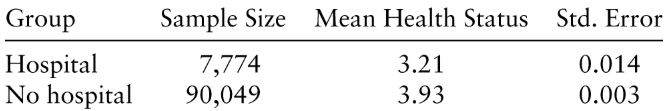
\includegraphics[scale=0.5]{Hospital}
\end{figure} 
\end{frame}

\begin{frame}
\frametitle{\: \: \: Randomization}
\toplinemedium
\begin{itemize}
\item The issue with using the survey is that individuals who are hospitalized are, on average, in much poor health (selection Bias)
\vspace{0.11in} 
\item We can also use regression analysis to study this issue:
\begin{eqnarray*}
y_i=\underbrace{\alpha}_{E[y_{0i}]}+\underbrace{\rho}_{y_{1i}-y_{0i}} \: D_i+\underbrace{\epsilon_i}_{y_{0i}-E[y_{0i}]}
\end{eqnarray*}
where
\begin{eqnarray*}
\begin{array}{ll}
E[y_i|D_i=1]= &\alpha+\rho+E[y_{0i}-E[y_{0i}]|D_i=1] \\[5ex]
E[y_i|D_i=0]= & \alpha+E[y_{0i}-E[y_{0i}]|D_i=0] 
\end{array}
\end{eqnarray*}
if randomly assigned:
\begin{eqnarray*}
E[y_{0i}-E[y_{0i}]|D_i=1]=E[y_{0i}-E[y_{0i}]|D_i=0]=0
\end{eqnarray*}
\end{itemize}
\end{frame}

\begin{frame}
\frametitle{\: \: \: Example: Project STAR}
\toplinelarge
\begin{figure}
\centering
\includegraphics[scale=0.5]{Star1}
\end{figure} 
\end{frame}


\begin{frame}
\frametitle{\: \: \: Example: Project STAR}
\toplinelarge
\begin{figure}
\centering
\includegraphics[scale=0.37]{Star2}
\end{figure} 
\end{frame}
\end{document}
